
\documentclass[11pt]{article}

\usepackage[square,sort,comma,numbers]{natbib}

\bibliographystyle{abbrvnat}
\setcitestyle{authoryear,open={(},close={)}}
\usepackage[utf8]{inputenc}
\usepackage{epsfig}
\usepackage{latexsym}
\usepackage{hyperref}
\usepackage{graphicx}
\usepackage[center]{caption}
%\usepackage{refcheck}
\DeclareGraphicsExtensions{.pdf,.png,.jpg}
\captionsetup{justification=centering,margin=2cm}
\begin{document}

	\title{Research Proposal}

	\author{Nirbhay P. Tandon\\MSc. Data Science\\
		Research Title:\\Develop New Transformer Architecture For \\ Question and Answering(QandA)
	}
	\date{}
	\maketitle

	\newpage
	\begin{abstract}
		Attention-based Transformer architectures have become the norm of current Natural Language Processing applications. Google began this trend back in 2017 with their paper \textit{Attention Is All You Need}, by introducing the Transformer architecture that works solely on attention mechanisms. The purpose of our work will be to create a new kind of Transformer architecture. Compare and contrast its performance against other architectures such as BERT, DistilBERT, ALBERT etc. using the SQuAD 2.0 Dataset. Through our research, we aim to produce a new architecture that has a better performance than existing models specifically for Question Answering based applications.
	\end{abstract}
	\newpage
	\tableofcontents
	\newpage
	\listoffigures
	\newpage
	\section{Introduction}\label{introduction}

	Question-Answering based systems have gained a lot of popularity, especially in the form of ``chatbots''. These systems depend highly on contextual understanding of the input, the training corpus and the question asked. They use this knowledge to output an answer that can help the user with whatever their query is. Recurrent neural networks and architectures based on them, have been able to provide great advancements in the field of Question-answering and chatbots in general. However, there is a behaviour of over-fitting and lack of contextual understanding of the question. This, coupled with long training times and extremely complex mathematical model designs, have often kept the field of Natural Language Processing slightly obscured from the masses.

	We wish to change that. Through our work, we would like to aim at creating a sustainable, fast, easy to understand Transformer architecture for Question Answering. An advancement on the work done by the team at Google \citep{atayl}. To be able to do so, let us first understand what a \textit{Transformer} is.
    A Transformer is a form of transduction model that relies solely on self-attention to figure out how to represent its inputs and outputs. It does so without the use of any sequence aligned recurrent neural networks(RNNs) or convolutions.

    Through our research proposal we wish to highlight why we are going to be performing this research and putting in the effort to devise a new architecture. We have divided our research proposal into 7 sections. In Section \ref{introduction}, we shall take a look at briefly introducing the concept and why our work is necessary. Next, in Section \ref{backRR}, we outline the background work that has already been done in this field and how some of the papers relate to the work that has been done. We use this as an opportunity to highlight some of the shortcomings in current architectures and modelling techniques. In Section \ref{aims}, we briefly outline the aim of our proposed research. In Section \ref{researchMeth}, we define in some detail the work that we will do to establish our research and how we plan to quantify the work that shall be done. Section \ref{expectedoutcomes}, highlights our goal, which is to produce a new transformer architecture that performs better at Question Answering based tasks.
	In Section \ref{resources}, we have outlined the minimum hardware requirements along with the resources available to the author that will be used to conduct this research. Finally, in Section \ref{plan}, we submit a Gantt Chart to outline our plan against the number of weeks.

	\section{Background and Related Research}\label{backRR}
	In this section, we shall highlight what has led us this far and some of the interesting challenges that it poses. In \ref{back}, we briefly look at the history of Natural Language Processing and how some of the challenges were addressed. In \ref{rr}, we look at the latest research that has gone into creating the Transformer architecture, identify some of the common patterns and use that information to strategise our model in later sections.

    \subsection{Background}\label{back}

	The area of Natural language Processing has taken significant leaps in the last two decades. Work done towards improving the ability of machine learning models to first recognize words, then sentences, followed by contextual understanding has led to several interesting and novel approaches in the field. From early on neural networks to creating Long Short-Term Memory architectures \citep{originallstm} by Sepp Hochreiter and Jurgen Schmidhuber in the mid-'90s that resolved the vanishing gradient problem of classical neural networks, we have come a long way.

	The latest advancements in this field come from Google's research lab in the form of \textit{Transformers}. We look into this in a bit more detail later. However, no model can be successful without a good dataset to train on. This is where the SQuAD 2.0 dataset \citep{dataset} comes in. This dataset is what forces the machine learning models to do contextual understanding. One might even say that it forces the models to ``think'' for themselves before answering a task.

    Let us now look at some of the key research that has been done in this regard.

	\subsection{Related Research}\label{rr}
	Outlined below are some of the most important pieces of research that relate directly to the work done for Transformers and Q\&A based systems.
	\begin{enumerate}
		\item The SQuAD 2.0 Dataset \citep{dataset}, was developed with funding from Facebook to help address some major issues with existing datasets. Most datasets focus on questions that can be easily answered or use of automatically generated, unanswerable questions which are easily identifiable.\\
		The SQuAD 2.0 dataset resolves this by combining the SQuAD dataset along with 50,000 crowd worker generated unanswerable questions. The key feature of these being that the unanswerable questions must look similar to answerable ones. For a model to be successful on this new dataset, it must be able to answer all possibly answerable questions as well as determine when no answers are provided for a question in the given paragraph and abstain from answering. A comparative study was done for a Natural Language Understanding(NLU) task that obtained an 86\% score on SQuAD 1.1, only got 66\% on the new 2.0 dataset.
		The dataset helps bridge the gap between true NLU and machine understanding by using the concept of Relevance. Through comparisons with various datasets such as RACE, MCTest, QASENT etc. they have identified the missing links like negative examples, antonyms and helped fill the gap. This dataset forces the models to understand whether a paragraph span has the answer to the question posed.

		\item Work done in the field of Long short-term and gated recurrent \citep{lstm} and \citep{recurrent} neural networks, in particular, has been established as a state of the art approach in sequence modelling, transduction problems such as language modelling and machine translation.
		In their paper Attention Is All You Need,\citep{atayl} the team set out to resolve problems in the parallelization and increased compute times of recurrent models. The inherently sequential nature of RNNs causes issues in memory constraints, leading to reduced batch sizes.\\
		\begin{figure}[h!]
			\centering
			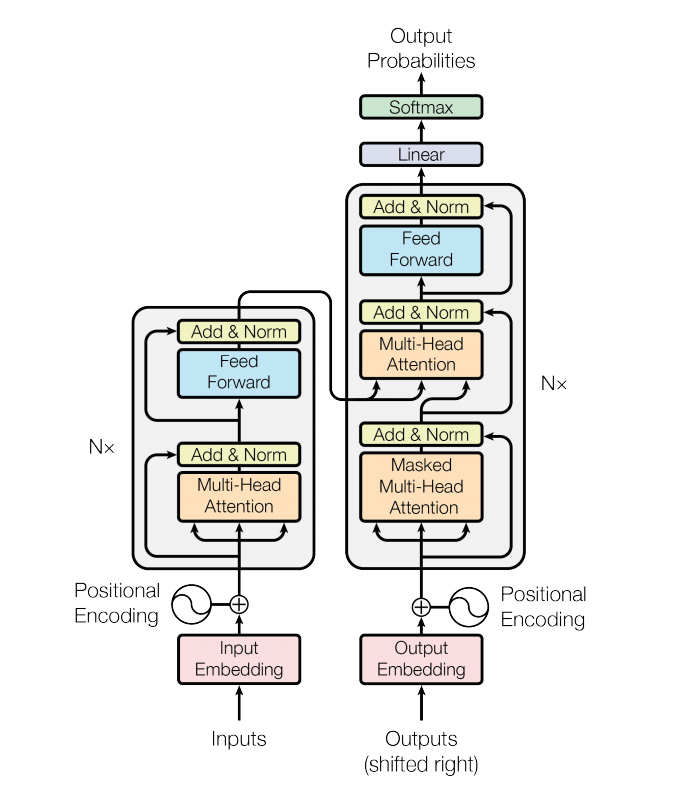
\includegraphics[scale=0.25]{transformer.png}
			\label{fig1}
			\caption{Transformer Architecture built by \citep{atayl}}
		\end{figure}
		The architecture for a \textit{Transformer} in this paper is outlined as having an encoder that maps input sequences to a continuous representation. The architecture can be seen above in Figure 1. This is then decoded into an output sequence of symbols one at a time. Each step is auto-regressive, i.e. it consumes the previously generated symbols as additional input when creating the next. This is similar to an ensemble model. Stacks of 6 encoder layers and 6 decoder layers is used.\\
		The encoder layers each have 2 sub-layers of a multi-head self-attention and the other a simple, position-wise fully connected feed-forward network layer.\\
		The decoder layer is similar to the encoder layer and has an additional 3rd sub-layer that performs multi-head attention over the output of the encoders. There is also normalization and  the outputs are prevented from attending to subsequent positions. \\ The attention mechanism can be described as mapping a query to a set of key-value pairs. This can be seen from Figure 2, below. \\The evaluations performed on the Wall Street Journal dataset\citep{wsj}, using 40k sentences, showed that even without task-specific tuning the model had better results with a fraction of the training cost.
		  \begin{figure}[h!]
        	\centering
        	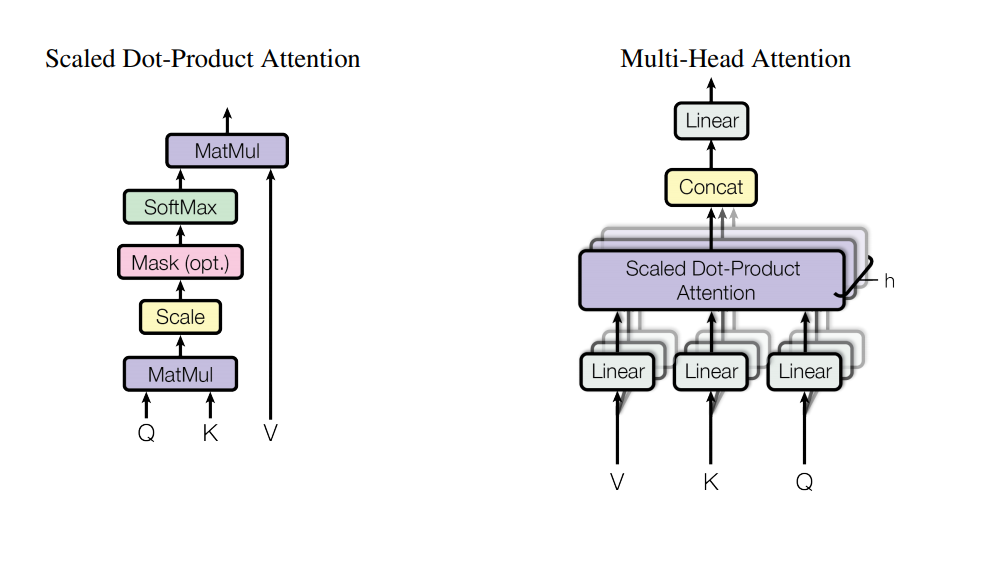
\includegraphics[scale=0.4]{multihead.png}
        	\label{fig2}
        	\caption{Scale Dot and Multihead Attention Models \cite{atayl}}
          \end{figure}
		\item The paper on BERT, which is \textit{Bidirectional Encoder Representations from Transformers} \citep{bert}, introduces a new language model. This model is truly fascinating in many ways. First and foremost it is designed to pre-train deep bidirectional representations using unlabelled data. This is done by jointly conditioning context in all layers to the right and left. This pre-training allows the model to be fine-tuned simply using one additional output layer. These features make this model conceptually simple and very powerful empirically.

        BERT employs language pre-training \citep{dai} which has shown significant advantages in many applications e.g. paraphrasing, language level inference etc. These tasks aim to highlight the relationships between sentences through contextual understanding as well as by using tokenized outputs.
        \begin{figure}[h!]
            \centering
            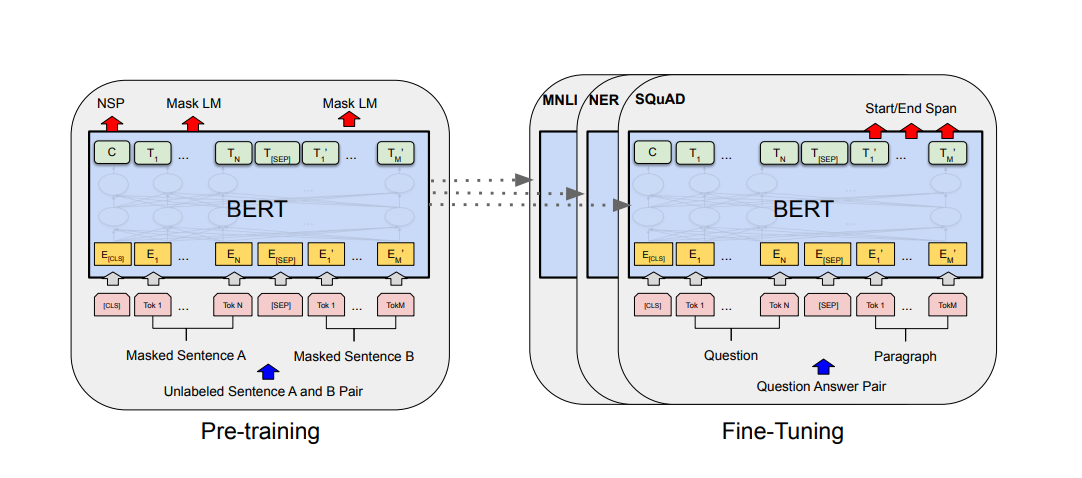
\includegraphics[scale=0.35]{BERT.png}
            \label{fig3}
            \caption{Pre-training and Fine Tuning procedures for BERT \citep{bert}}
        \end{figure}

        BERT was tested on The General Language Understanding Evaluation (GLUE) benchmark \citep{wang} which has a large number of diverse NLU tasks.
		BERT performed extremely well on the 11 NLP tasks that the authors ran it against. it showed an average accuracy improvement of 4.5\% and 7\% when compared to the previous state of the art models. Results of BERT and its significant gains make it one of the best candidate models for NLU tasks.

	\end{enumerate}

    Several advancements have been made to the BERT model to make it fast, better at understanding and even performing application-specific tasks such as Q\&A.

    The SQuAD 2.0 dataset has inspired an LSTM based FastQA \citep{fastQA} model architecture. This architecture takes cues from the work done by Hochreiter and Schmidhuber in their work on Long Short-Term Memory Architecture \citep{lstm}, to create a model specifically for end-to-end question answering systems.

    A common theme with BERT is that it takes a long time to train. Especially in the BERT based RoBERTa architecture \cite{roberta}. RoBERTa takes on average 4-5 times more time to train than BERT, however, it also shows a maximum of 20\% improvement over BERT, depending on the application. ALBERT, which is A Liter BERT, \cite{albert} was developed specifically to deal with memory limitations and reduce training times. ALBERT's XXL implementation has been documented to perform better in models trained on the BOOKCORPUS and Wikipedia ones by at least 2\% across multiple applications. In a smaller amount of time.

    However, none of these model architectures has been able to address all the problems and serve as more generic solutions to multiple end-to-end sequence encoding problems across various applications.

    Our work is primarily focused on building a fast model that allows for higher accuracy in responses specifically with Q\&A systems.

	\section{Aims and Objectives}\label{aims}

	The main aim of this research is to propose a new transformer architecture that can perform better at Q\&A using the SQuAD 2.0 dataset.
	We shall:
	\begin{enumerate}
		\item Implement the existing models that are available via libraries such as HuggingFace \citep{hfTransformers}, PyTorch and Tensorflow on the dataset
		\item Obtain F1, validation, etc. scores for existing models and treat them as our benchmark scores
		\item Identify drawbacks of the current architectures
		\item Design our architecture and evaluate its performance
		\item Fine-tune the architecture, re-evaluate and report improvements
		\item Compare the results of our Transformer model with the benchmark scores.
	\end{enumerate}

	\section{Research Methodology}\label{researchMeth}

	To implement this research we shall break the project down into 5 phases. These are outlined below.
	\subsection{Research Dataset}\label{datas}

	We have selected the Stanford Question Answering Dataset (SQuAD). This is as a reading comprehension dataset based on Wikipedia articles. It is based on questions posed by crowd-workers on a set of articles. The answer to every question is a segment of text or span, from the corresponding reading passage, or the question might be unanswerable \citep{dataset}.

	The dataset consists of over 150,000 questions. Split into 100,000 answerable and 50,000+ unanswerable question, which were written to look similar to unanswerable questions. The challenge being that a model should be able to correctly answer the answerable questions and abstain from answering the unanswerable ones.
	The dataset is freely available as a part of the Transformers package in python or it can be downloaded from the SQuAD 2.0 website \citep{squad}.

	To effectively use this dataset for our purposes, let us first take a look at what its contents look like below.\\ \\
	\noindent\fbox{
	\parbox{\textwidth}{\textbf{Context: } \textit{"The Normans (Norman: Nourmands; French: Normands; Latin: Normanni) were the people who in the 10th and 11th centuries gave their name to Normandy, a region in France. They were descended from Norse ("Norman" comes from "Norseman") raiders and pirates from Denmark, Iceland and Norway who, under their leader Rollo, agreed to swear fealty to King Charles III of West Francia."}\\
		\textbf{Question: } \textit{Who was the Norse leader?}\\
		\textbf{Answer: } \textit{Rollo}}
	}
	\\ \\

	The answer to the aforementioned question is quite simple for humans to comprehend. The challenge is for us to contextualize this and make it machine-understandable so that our model can answer it correctly.

	The dataset consists of various kinds of English language examples like negation, antonyms, entity swaps, impossible conditions to answer, answerable, etc. making the dataset a well-balanced one.

	To use this dataset correctly we shall perform the following pre-processing steps on it:

	\begin{enumerate}
		\item Data splitting into separate Question, Answer and Context lists.
		\item Splitting the data into separate training and validation sets of  question and answers using the 80/20 rule, also known as the Pareto principle. We will have 80\% training data and 20\% test data.
		\item Tokenization of the split data to generate "context-question" pairs
		\item Generating indexes for when an answer begins and ends in the dataset
		\item Adding answer tokens based on their encoded positions
	\end{enumerate}
	\subsection{Research Benchmarks}\label{benchmarks}
	Here we shall focus on obtaining benchmark scores for the shortlisted architectures i.e BERT \citep{bert}, DistilBERT \citep{distil} and ALBERT \cite{albert}, on the above dataset.

	We shall use the F1, Exact Match(EM), Recall and Training Time scores to create a benchmark to compare our architecture against. The Exact Match score will help us identify how many questions were 100\% correctly answered by each model.

	\subsection{Architecture Creation}\label{architecturecreation}
	In this section we will:

	\begin{enumerate}
		\item{Mathematically model a new transformer architecture}
		\item{Code the architecture}
		\item{Run sample dataset to identify base benchmarks}
		\item{Run the SQuAD 2.0 dataset to obtain 1st pass performance benchmarks}
		\item{Document architecture performance, identify pros and cons}
	\end{enumerate}
	\subsection{Architecture Refinement}\label{refinement}
	In this phase, we will focus on:
	\begin{enumerate}
		\item{Reviewing the results from the previous section}
		\item{Identifying the areas of improvement}
		\item{Hypothesise the improvements and implement them in the architecture}
		\item{Run the SQuAD 2.0 dataset to obtain new performance benchmarks}
		\item{Document architecture performance, identify pros and cons}
	\end{enumerate}
	\subsection{Model Evaluation}
	The training shall be carried out using the train-test loss plot to identify the optimal number of epochs for which our model needs to be run. This will also be done for the selected model architectures.

    The main parameters we will use for model evaluation are F1, Exact Match(EM), Recall and Training Time.

    These metrics will help us reiterate and quantify correctly if our model has improved performance or not.

	\section{Expected Outcomes}\label{expectedoutcomes}

	We expect that our created model is at-par, if not better, at performing Q\&A than existing models.
	\section{Requirements and Resources}\label{resources}

	To successfully deliver on our research we will be utilizing the following hardware:
	\begin{itemize}
		\item EVGA GeForce RTX 2070 SUPER KO GAMING, 08G-P4-2072-KR, 8GB GDDR6, Dual Fans\citep{evga}. This graphics card is based on the Nvidia "Turing" architecture and has 2560 CuDA cores.
		\item Intel 10700 processor. 8 cores, 16 threads, 16M cache\citep{intel}.
		\item VENGEANCE® LPX 8GB (1 x 8GB) DDR4 DRAM 2400MHz C14 Memory Kit - Black\citep{Ram}. 8GB x 4, 32 GB total.
		\item Ubuntu 20.04 Operating System
		\item We will also be using the latest versions of the following packages: Pandas, NumPy, SciPy, Transformers by HuggingFace, Matplotlib, Tensorflow and PyTorch. In case there are compatibility issues the appropriate versions will be mentioned. We will also mention any other packages that might be required in the course of the research.
	\end{itemize}


	The above hardware is available to the author and any changes to the same will be notified/highlighted in the subsequent reports.
	\section{Research Plan}\label{plan}

	Shown on the next page is the Gantt Chart highlighting the research stages and timelines.\\
	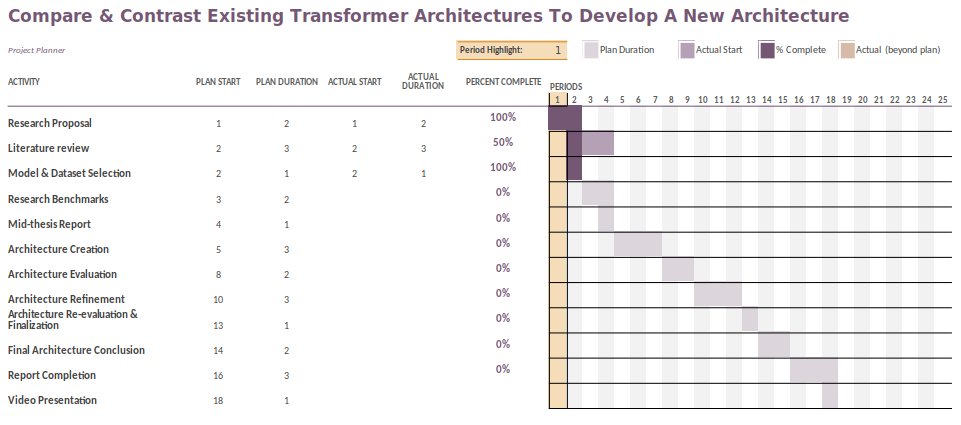
\includegraphics[width=180mm,height=120mm,angle=90]{g2.png}
	\newpage
	\bibliography{Research_Proposal}

\end{document}
